\begin{table}[t]
    \small
    \begin{center}
    \caption{\it Geometry of a measured trombone taken from \cite{Smyth2011}. Numbers correspond to Figure \ref{fig:tromboneSchematic}.\label{tab:geometry}}
    \begin{tabular}{|l|c|c|}
        \hline
        Part of tube & Length (cm) & Radius (cm)\\\hline
        Inner slide (1) & 70.8 & 0.69\\
        Outer slide (extended) (2) & 53 & 0.72 
        \\
        Slide crook (3)& 17.7 & 0.74\\
        Outer slide (extended) (4) & 53 & 0.72 
        \\
        Inner slide (5) & 71.1 & 0.69\\
        Gooseneck (6) & 24.1 & 0.71\\
        Tuning slide (7) & 25.4 & 0.75, 1.07\\
        Bell flare (8) & 50.2& 1, 10.8\\\hline
    \end{tabular}
    \end{center}
\end{table}

\begin{table}[t]
    \small
    \begin{center}
    \caption{\it List of parameter values used for the simulation. 
    Taken from $^\star$\cite{Smyth2011}, *\cite{Harrison2018} or **\cite{Benade1968} with temperature $T=26.85^\circ C$. \label{tab:parameters}}
    \begin{tabular}{|l|c|c|}
        \hline
        Name & Symbol (unit) & Value\\ \hline
        \multicolumn{3}{|l|}{\bf Tube}\\ \hline
        Length & $L$ (m) & $2.593\leq L \leq 3.653$$^\star$\\
        Air density &$\rho_0$ (kg/m$^3$) & 1.1769** 
        \\
        Wave speed & $c$ (m/s) & 347.23**\\
        Geometry & $S$ (m$^2$) & See Table \ref{tab:geometry}. \\\hline
        \multicolumn{3}{|l|}{\bf Lip reed}\\ \hline
        Mass & $M_\text{r}$ (kg) & $5.37\cdot10^{-5}$*\\
        Frequency & $\omega_\text{r}$ (rad/s) & $ 20\leq \omega_\text{r}/2\pi \leq 1000$\\
        Mouth pressure & $P_\text{m}$ (Pa) & $0 \leq P_\text{m} \leq 6000$\\
        Damping & $\sigma_\text{r}$ (s$^{-1}$) & $5$*\\
        Eff. surface area & $S_\text{r}$ (m$^{2}$) & $1.46\cdot 10^{-5}$*\\
        Width & $w_\text{r}$ (m) & $0.01$* \\
        Equilibrium sep. & $H_0$ (m) &  $2.9 \cdot 10^{-4}$* \\
        Coll. stiffness& $K_\text{c}$ (N/m) & $10^4$\\
        Nonlin. coll. coeff.& $\alpha_\text{c}$ (-)  &3\\\hline
        \multicolumn{3}{|l|}{\bf Other}\\ \hline
        % State corr. stiffness & $\omega_\text{sc}$ & $1$\\ 
        State corr. damping & $\sigma_\text{sc}$ & $1$\\ 
        Sample rate & $f_\text{s}$ (Hz) & 44100\\
        \hline
    \end{tabular}
    \end{center}
\end{table}
\begin{figure}[ht]
    \centering
    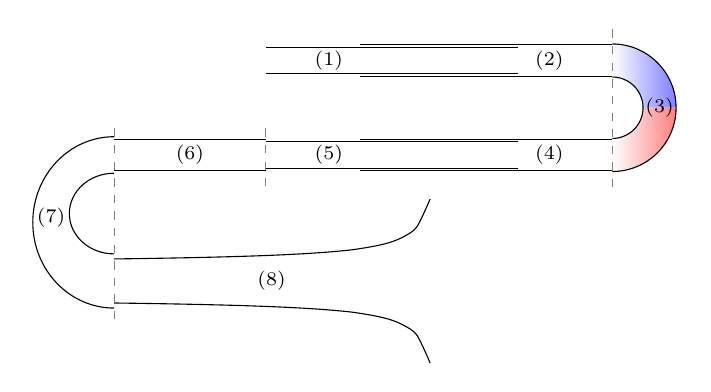
\begin{tikzpicture}[scale = 8]

    \def\labelColor{black};
    \def\labelSize{\fontsize{7pt}{7pt}\selectfont};

    \def\hornOffset{0.025};
    \def\stepSize{0.004}

    \def\dashedLineColor{gray};
    \def\dashedLineOvershoot{0.025}
    % tuning slide params
    \def\tuningSlideDim{0.1};
    \pgfmathsetmacro{\tuningSlideRad}{\stepSize + \hornOffset};
    \def\tuningSlideOffset{0.007};

    % gooseneck params
    \def\gooseNeckLength{0.241};
    \pgfmathsetmacro{\gooseNeckRad}{\tuningSlideRad - \stepSize};

    % inner slide params
    \def\innerLength{0.4};
    \pgfmathsetmacro{\innerRad}{\gooseNeckRad - \stepSize};

    % outer slide params
    \def\outerLength{\innerLength};
    \pgfmathsetmacro{\outerRad}{\gooseNeckRad};
    \pgfmathsetmacro{\extension}{0.15};

    \def\endOfSlideDim{0.075};
    \pgfmathsetmacro{\endOfSlideRad}{\outerRad * 1.05};

    %% draw horn

    \draw[domain=0:0.502, smooth, variable=\x, black] plot ({\x}, {\hornOffset + 0.0063 * ((0.502-\x) + 0.0174)^(-0.7)});
    
    \draw[domain=0:0.502, smooth, variable=\x, black] plot ({\x}, {-\hornOffset-0.0063 * ((0.502-\x) + 0.0174)^(-0.7)});
    
    \node[anchor = center, color = \labelColor](eight) at (0.25, 0) {\labelSize(8)};

    % draw tuningSlide
    \pgfmathsetmacro{\innerTuningSlideDim}{(\tuningSlideDim - \tuningSlideRad)}
    \pgfmathsetmacro{\outerTuningSlideDim}{(\tuningSlideDim + \tuningSlideRad)}

    \node[anchor = center, color = \labelColor](seven) at (-\innerTuningSlideDim-\tuningSlideRad, \innerTuningSlideDim+\tuningSlideRad) {\labelSize(7)};

    \pgfmathsetmacro{\innerTuningSlideWithOffset}{\innerTuningSlideDim - \tuningSlideOffset}

    \pgfmathsetmacro{\outerTuningSlideWithOffset}{\outerTuningSlideDim + \tuningSlideOffset}

    \draw (0, 2*\tuningSlideDim-\tuningSlideRad) arc(90:270:\innerTuningSlideDim cm and \innerTuningSlideWithOffset cm);

    \draw (0, 2*\tuningSlideDim+\tuningSlideRad) arc(90:270:\outerTuningSlideDim cm and \outerTuningSlideWithOffset cm);
    
    % dashedline
    \draw[dashed, color = \dashedLineColor] (0, -\tuningSlideRad-\tuningSlideOffset-\dashedLineOvershoot) -- (0, 2*\tuningSlideDim+\tuningSlideRad+\dashedLineOvershoot);

    % draw gooseneck
    \draw (0, 2*\tuningSlideDim + \gooseNeckRad) -- (\gooseNeckLength, 2*\tuningSlideDim + \gooseNeckRad);

    \draw (0, 2*\tuningSlideDim - \gooseNeckRad) -- (\gooseNeckLength, 2*\tuningSlideDim - \gooseNeckRad);

    \node[anchor = center, color = \labelColor](six) at (0.5 * \gooseNeckLength, 2*\tuningSlideDim) {\labelSize(6)};

    % dashedline
    \draw[dashed, color = \dashedLineColor] (\gooseNeckLength, 2*\tuningSlideDim-\gooseNeckRad-\dashedLineOvershoot) -- (\gooseNeckLength, 2*\tuningSlideDim+\gooseNeckRad+\dashedLineOvershoot);

    % draw inner slide
    \draw (\gooseNeckLength, 2*\tuningSlideDim + \innerRad) -- (\gooseNeckLength+\innerLength, 2*\tuningSlideDim + \innerRad);

    \draw (\gooseNeckLength, 2*\tuningSlideDim - \innerRad) -- (\gooseNeckLength+\innerLength, 2*\tuningSlideDim - \innerRad);

    \node[anchor = center, color = \labelColor](five) at (\gooseNeckLength + 0.25 * \innerLength, 2*\tuningSlideDim) {\labelSize(5)};

    % draw outer slide
    \pgfmathsetmacro{\outerSlideStart}{\gooseNeckLength + \extension};

    \draw (\outerSlideStart, 2*\tuningSlideDim + \outerRad) -- (\outerSlideStart+\outerLength, 2*\tuningSlideDim + \outerRad);

    \draw (\outerSlideStart, 2*\tuningSlideDim - \outerRad) -- (\outerSlideStart+\outerLength, 2*\tuningSlideDim - \outerRad);

    \node[anchor = center, color = \labelColor](four) at (\outerSlideStart + 0.75 * \outerLength, 2*\tuningSlideDim) {\labelSize(4)};


    % draw end of slide
    
    \pgfmathsetmacro{\innerEndOfSlideDim}{(\endOfSlideDim - \endOfSlideRad)};
    \pgfmathsetmacro{\outerEndOfSlideDim}{(\endOfSlideDim + \endOfSlideRad)};

    \pgfmathsetmacro{\startEndOfSlide}{\outerSlideStart + \outerLength};
    % division blue
    \fill[white, left color=white, right color=blue, fill opacity = 0.5] 
    (\startEndOfSlide+\innerEndOfSlideDim,2*\tuningSlideDim+\endOfSlideDim) 
    arc (0:90:\innerEndOfSlideDim cm and \innerEndOfSlideDim cm) 
    -- (\startEndOfSlide,2*\tuningSlideDim+\endOfSlideDim + \innerEndOfSlideDim)
    -- (\startEndOfSlide,2*\tuningSlideDim+2*\endOfSlideDim+\endOfSlideRad)
    arc (90:0:\outerEndOfSlideDim cm and \outerEndOfSlideDim cm)
    -- (\startEndOfSlide+\outerEndOfSlideDim,2*\tuningSlideDim+\endOfSlideDim)
    -- cycle;

    % division red
    \fill[white, left color=white, right color=red, fill opacity = 0.5] 
    (\startEndOfSlide+\innerEndOfSlideDim,2*\tuningSlideDim+\endOfSlideDim) 
    arc (0:-90:\innerEndOfSlideDim cm and \innerEndOfSlideDim cm) 
    -- (\startEndOfSlide,2*\tuningSlideDim+\endOfSlideDim)
    -- (\startEndOfSlide,2*\tuningSlideDim-\endOfSlideRad)
    arc (-90:0:\outerEndOfSlideDim cm and \outerEndOfSlideDim cm)
    -- (\startEndOfSlide+\outerEndOfSlideDim,2*\tuningSlideDim+\endOfSlideDim)
    -- cycle;

    \draw (\startEndOfSlide, 2*\tuningSlideDim+\endOfSlideRad) arc(-90:90:\innerEndOfSlideDim cm and \innerEndOfSlideDim cm);

    \draw (\startEndOfSlide, 2*\tuningSlideDim-\endOfSlideRad) arc(-90:90:\outerEndOfSlideDim cm and \outerEndOfSlideDim cm);

    \node[anchor = center, color = \labelColor](three) at (\startEndOfSlide + \innerEndOfSlideDim + \endOfSlideRad, 2*\tuningSlideDim+ \innerEndOfSlideDim + \endOfSlideRad) {\labelSize(3)};


    % dashedline
    \draw[dashed, color = \dashedLineColor] (\startEndOfSlide, 2*\tuningSlideDim-\endOfSlideRad-\dashedLineOvershoot) -- (\startEndOfSlide, 2*\tuningSlideDim+2*\endOfSlideDim+\endOfSlideRad+\dashedLineOvershoot);

    % draw second outer slide

    \draw (\outerSlideStart, 2*\tuningSlideDim + 2 * \endOfSlideDim + \outerRad) -- (\outerSlideStart+\outerLength, 2*\tuningSlideDim + 2 * \endOfSlideDim + \outerRad);

    \draw (\outerSlideStart, 2*\tuningSlideDim + 2 * \endOfSlideDim - \outerRad) -- (\outerSlideStart+\outerLength, 2*\tuningSlideDim + 2 * \endOfSlideDim - \outerRad);

    \node[anchor = center, color = \labelColor](two) at (\outerSlideStart + 0.75 * \outerLength, 2*\tuningSlideDim + 2 * \endOfSlideDim) {\labelSize(2)};

    % draw inner slide
    \draw (\gooseNeckLength, 2*\tuningSlideDim+ 2 * \endOfSlideDim + \innerRad) -- (\gooseNeckLength+\innerLength, 2*\tuningSlideDim+ 2 * \endOfSlideDim + \innerRad);

    \draw (\gooseNeckLength, 2*\tuningSlideDim + 2 * \endOfSlideDim - \innerRad) -- (\gooseNeckLength+\innerLength, 2*\tuningSlideDim + 2 * \endOfSlideDim - \innerRad);

    \node[anchor = center, color = \labelColor](one) at (\gooseNeckLength + 0.25 * \innerLength, 2*\tuningSlideDim + 2 * \endOfSlideDim) {\labelSize(1)};

% \begin{scope}[very thick,decoration={
%     markings,
%     mark=at position 0.5 with {\arrow{>}}}
%     ] 
%     \draw[postaction={decorate}] (-4,0)--(4,0);
% \end{scope}
    
    \end{tikzpicture}
    \caption{Schematic of the trombone. Numbers correspond to the parts of the tube found in Table \ref{tab:geometry} and dashed lines highlight where parts are separated. The scheme is split in the middle of the slide crook with the colours corresponding to those in \ref{fig:dynamicGridSchematic}.}
    \label{fig:tromboneSchematic}
\end{figure}

\section{Implementation}\label{sec:implementation}
The implementation has been done in C++ using the JUCE framework \cite{JUCE}, and is available online\footnote{\href{https://github.com/SilvinWillemsen/cppBrass/releases/tag/v1.0}{https://github.com/SilvinWillemsen/cppBrass/releases/}} as well as a demo showcasing it.\footnote{\href{https://youtu.be/Ht5gVNrshYo}{https://youtu.be/Ht5gVNrshYo}} The audio output of the system can be retrieved by selecting one or multiple grid points on the pressure grid and listening to this at the given sample rate $f_\text{s}$. Here, the output is taken as the weighted average of the rightmost points until 10.8 cm (radius of the flare-end) from the end of the the radiating boundary. This range was chosen due to the fact that in the real world, the sound does not originate from a single point-like source, but rather from a larger -- here assumed to be spherical -- region of space. The spatial averaging has a low-passing effect on the sound, but informal listening tests by the authors have confirmed that the sound is more true to that of an actual trombone than if a single point is chosen. %To mimic high-frequency losses happening when the sound of the trombone travels from the bell to the ear, a 4\textsuperscript{th}-order low-passing Butterworth filter with a cutoff frequency of $0.05 f_\text{s}$ Hz is used.  

% We continue by providing the parameter values used in the simulation.
\subsection{Parameters}
For the most part, the parameters used in the simulation have been obtained from \cite{Harrison2018, Smyth2011, Benade1968}. The lengths and radii of different parts of the tube can be found in Table \ref{tab:geometry} and a diagram showing this geometry is shown in Figure \ref{fig:tromboneSchematic}.
The system is split in the middle of the slide crook such that the ranges for the lengths of the two tubes are $L_p^n \in[0.797, 1.327]$ and $L_q^n \in [1.796, 2.326]$.

Other parameters used in the simulation can be found in Table \ref{tab:parameters}. Not included here is $\lambda$, which has been set slightly lower than the stability condition in \eqref{eq:CFL}, i.e., $\lambda = 0.999$. Although the implementation works when $\lambda = 1$, this is done to tolerate (much) higher speeds of change in $L^n$ before instability occurs (see Section \ref{sec:limit}). Not satisfying condition \eqref{eq:CFL} causes bandlimiting and dispersive effects \cite{bilbao2009}, but such a small deviation from the condition has no perceptual influence on the output sound and outweighs the problems caused by instability.

As the tube acts mainly as an amplifier for specific resonant frequencies it is important to match the frequency of the lip reed to a resonating mode of the tube. This frequency depends on $L^n$ in the following way
\begin{equation}\label{eq:lipReedCalc}
    \omega_\text{r}^{n+1/2} = \mathcal{F}\frac{2\pi c}{\rho_0 L^{n+1/2}}\ ,
\end{equation}
where $L^{n+1/2} = L^n$ and scalar multiplier $\mathcal{F} = 2.4$ was heuristically found to best match the 4\textsuperscript{th} resonating mode of the tube and generates a recognisable brass sound.

\subsection{Limit on speed of change}\label{sec:limit}
To reduce audible artifacts and instability issues from adding and removing points, and to stay in the sub-audio rate regime, a limit can be placed on \eqref{eq:lDiff} as
\begin{equation}\label{eq:Nmaxdiff} 
    L_\text{diff}^n \leq \Nfrac_\text{maxdiff} h,
\end{equation}
where $\Nfrac_\text{maxdiff}$ is the maximum change in $\Nfrac$ per sample and has been set to $\Nfrac_\text{maxdiff} = 1/20$. This means that a grid point can be added or removed every 20 samples and allows the entire range of $L$ to be traversed in ca. 0.06 s at a sample rate of $f_\text{s} = 44100$ Hz.

\subsection{State correction}\label{sec:impStateCorr}
The introduction of system states at $n+1$ through the centred operators in Eq. \eqref{eq:scForce} seem to make the scheme implicit. It is, however, possible to calculate $F_\text{sc}$ explicitly \cite{bilbao2009, bilbao2009dafx}. The same operators also introduce the need for values at $n-1$, i.e., $p_{M^n}^{n-1}$ and $q_{0}^{n-1}$. Therefore, the vectors $\mathbf{p}^{n-1}$ and $\mathbf{q}^{n-1}$ will need to be stored, and the operations to add and remove grid points as described in \ref{sec:addRemove} need to be applied to these as well. One could argue that only two points at the inner boundaries are needed for the calculation and to create $\mathbf{r}$ in \eqref{eq:interpVecs} at $n-1$. For generality, we continue with the entire vectors defined over the same domains as $\mathbf{p}^n$ and $\mathbf{q}^n$ respectively. 
\begin{figure}[t]
    \centering
    \setlength{\fboxsep}{0pt} 
    \fbox{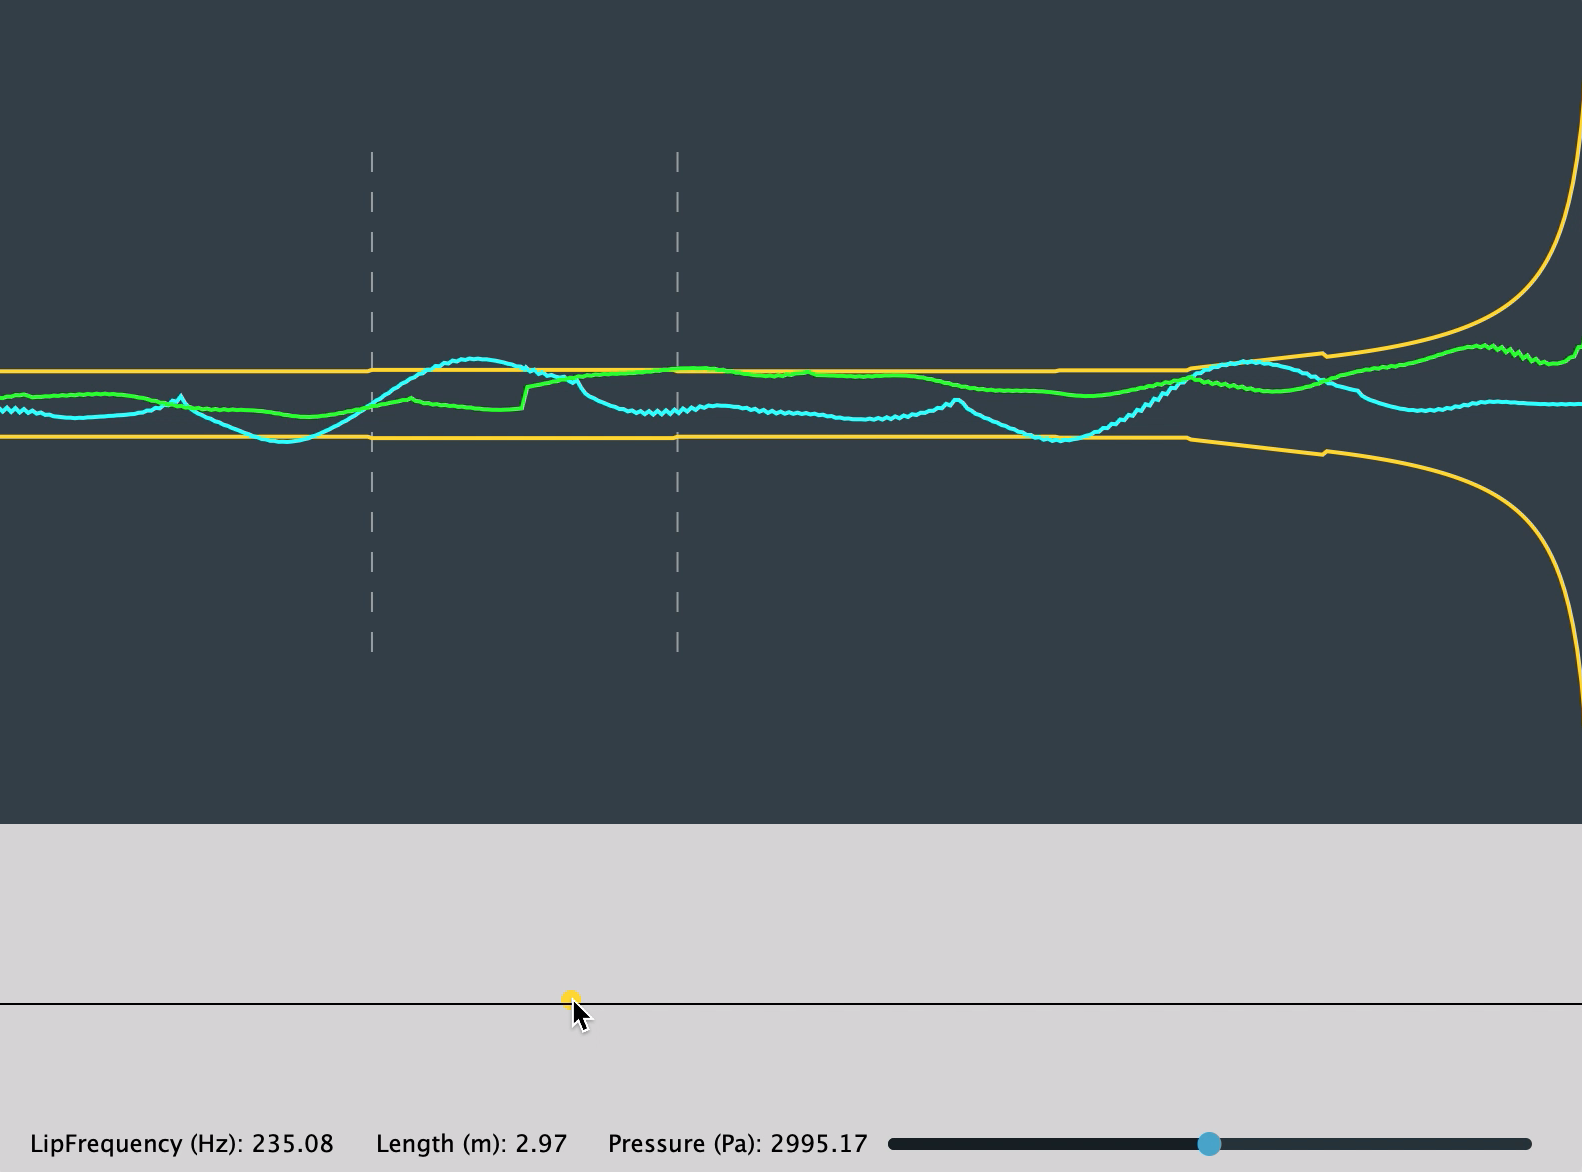
\includegraphics[width = \columnwidth]{Figures/GUI.png}}
    \caption{\it Screenshot of the graphical user interface (GUI). The geometry (in orange) as well as the states of the pressure (in blue) and velocity scaled by $S$ (in green) are shown. For clarity, the start and end of the outer slide are denoted by dashed lines. The drift of $w$ as explained in Section \ref{sec:drift} is visible from the ``kink'' in the green line exactly in the middle of the outer slide.}
    \label{fig:GUI}
\end{figure}

\subsection{Graphical User Interface and Control Mapping}
A screenshot of the graphical user interface (GUI) is shown in Figure \ref{fig:GUI}. The geometry of the tube is plotted along with paths showing the pressure states in blue and the velocity (scaled by the geometry $S$) in green. The audio thread of the application runs at 44100 Hz whereas the graphics are updated at a rate of 15 Hz. 

The real-time application is controlled by interacting with the bottom panel using the mouse. The x-axis is mapped to tube-length $L^n$ and also modifies the lip-reed frequency $\omega_\text{r}$ according to Eq. \eqref{eq:lipReedCalc}. The y-axis changes the multiplier $\mathcal{F}$ in Eq. \eqref{eq:lipReedCalc} and the black line in the vertical middle of the control panel is mapped to $\mathcal{F} = 2.4$. The pressure is modulated by a slider at the bottom of the control panel. As of now, no focus has been put on intuitive parameter mapping; it has only been implemented for simple parameter exploration.

% \begin{algorithm}[ht]
%     \setstretch{1.1}
%     \fbox{\parbox{0.88\linewidth}
%     {
%         \While{application is running}
%         {
%             Retrieve new parameters ($L^n$, $\omega_\text{r}^n$ and $P_\text{m}^n$) \\
%             Update $L_p^n$ and $L_q^n$ (Eqs. \eqref{eq:lDiff}, \eqref{eq:Nmaxdiff} and \eqref{eq:updateLs})\\
%             Calc. $\Nfrac^n$ and $N^n$ (Eqs. \eqref{eq:nfrac} and \eqref{eq:numberOfIntervals}) \\
%             Calc. $\alpha$ (Eq. \eqref{eq:alphaDef})\\
%             \If{$ N^n \neq N^{n-1} $}
%             {
%                 Add or remove point (Eq. \eqref{eq:addingPoint} or \eqref{eq:removingPoint})\\
%                 Update $M$ and $M_q$ (Eq. \eqref{eq:MMq})
%             }
%             Calc. $p_{M+1}^n$ and $q_{-1}^n$ (Eqs. \eqref{eq:connectionInterpol})\\
%             Calc. $\mathbf{v}^{n+1/2}$ and  $\mathbf{w}^{n+1/2}$ (Eqs. \eqref{eq:discVelocityV} and \eqref{eq:discVelocityW})\\
%             Calc. $y^{n+3/2}$ w/o collision (Eqs. \eqref{eq:discreteLipSystem})\\
%             Calc $g^{n+1/2}$ (Eq. \eqref{eq:gDef})\\
%             Calc. $y^{n+3/2}$ with collision (Eqs. \eqref{eq:discreteLipSystem})\\
%             Calc. $U_\text{B}^{n+1/2}$ and $U_\text{r}^{n+1/2}$ (Eqs. \eqref{eq:bernoulli} and \eqref{eq:Ur})\\
%             Calc. $\mathbf{p}^{n+1}$ and $\mathbf{q}^{n+1}$ (Eqs. \eqref{eq:pressuresWithSC})\\ 
%             Retrieve output\\
%             Update system states ($\mathbf{p}^{n-1} = \mathbf{p}^{n}$, $\mathbf{p}^n=\mathbf{p}^{n+1}$)\\
%             (same for $\mathbf{v}^{n-1/2} = \hdots$, $y^{n-1/2}$, $y^{n+1/2}$, and $\psi^n$),\\
%             % \begin{minipage}[c]{0.4\linewidth} 
%             % Update system states\\
%             % \\
%             % \\
%             % \\
%             % \end{minipage} \begin{minipage}[c]{0.5\linewidth} 
%             % $\mathbf{p}^{n-1} = \mathbf{p}^n$, $\mathbf{p}^n = \mathbf{p}^{n+1}$,\\
%             % $\mathbf{v}^{n-1/2} = \mathbf{v}^{n+1/2}$,\\
%             % $y^{n-1/2} = y^{n+1/2}$,\\
%             % $y^{n+1/2} = y^{n+3/2}$, \\
%             % $\psi^{n} = 
%             % \psi^{n+1}$, 
%             % \end{minipage}\\
%             Update $N$ ($N^{n-1} = N^n$)\\
%             Increment $n$            % \begin{minipage}[c]{0.4\linewidth}
%             % -\\
%             % \vspace{2em}(Eq. \eqref{eq:addingPoint})\\
            
%             % (Eq. \eqref{eq:removingPoint})\\

%             % \end{minipage}
%             }
%         }
%     }
%     \vspace{0.12cm}
%     \caption{Pseudocode showing the order of calculations of the algorithm implementing the trombone .\label{alg:calcOrder}}
% \end{algorithm}
\begin{algorithm}[t]
    \setstretch{1.1}
    \fbox{\parbox{0.88\linewidth}
    {
        \While{application is running}
        {
            \begin{minipage}[c]{0.48\linewidth}
                Retrieve new parameters\\
                Update $L_p^n$ and $L_q^n$\\
                Calc. $\Nfrac^n$ and $N^n$\\
                Calc. $\alpha^n$ \\
                \If{$ N^n \neq N^{n-1} $}
                {
                    Add or remove point\\
                    Update $M^n$ and $M_q^n$ 
                }
                Calc. $p_{M^n+1}^n$ and $q_{-1}^n$ \\
                Calc. $\mathbf{v}^{n+1/2}$ and  $\mathbf{w}^{n+1/2}$ \\
                Calc. $y^{n+3/2}$ w/o collision \\
                Calc $g^{n+1/2}$ \\
                Calc. $y^{n+3/2}$ with collision \\
                Calc. $U_\text{B}^{n+1/2}$ and $U_\text{r}^{n+1/2}$ \\
                Calc. $\mathbf{p}^{n+1}$ and $\mathbf{q}^{n+1}$ \\
                Retrieve output
            \end{minipage}
            \begin{minipage}[c]{0.43\linewidth}
                ($L^n$, $\omega_\text{r}^n$ and $P_\text{m}^n$) \\
                (Eqs. \eqref{eq:lDiff}, \eqref{eq:Nmaxdiff} \& \eqref{eq:updateLs})\\
                (Eqs. \eqref{eq:nfrac} and \eqref{eq:orderOfCalcGrid})\\
                (Eq. \eqref{eq:alphaDef})\\
                \vspace{-0.2em}\\
                (Eq. \eqref{eq:addingPoint} or \eqref{eq:removingPoint})\\
                (Eq. \eqref{eq:MMq})\\
                \vspace{-0.15em}\\
                (Eqs. \eqref{eq:connectionInterpol})\vspace{0.05em}\\
                (Eqs. \eqref{eq:discVelocityV} and \eqref{eq:discVelocityW})\\
                (Eqs. \eqref{eq:discreteLipSystem})\\
                (Eq. \eqref{eq:gDef})\\
                (Eqs. \eqref{eq:discreteLipSystem})\\
                (Eqs. \eqref{eq:bernoulli} and \eqref{eq:Ur})\\
                (Eqs. \eqref{eq:pressuresWithSC})
                \vspace{0.25em}\\
           \end{minipage}
           \\
           \begin{minipage}[c]{0.4\linewidth}
                Update system states\\
                \\
                \\
                Update $N^{n-1}$ \\
                Increment $n$      
            \end{minipage}
            \begin{minipage}[c]{0.5\linewidth}
                ($\mathbf{p}^{n-1} = \mathbf{p}^{n}$, $\mathbf{p}^n=\mathbf{p}^{n+1}$)
                (same for $\mathbf{v}^{n-1/2} = \hdots$,\\
                $y^{n-1/2}$, $y^{n+1/2}$, and $\psi^n$)\\
                ($N^{n-1} = N^n$)\\
            \end{minipage}
            }
        }
    }
    \vspace{0.12cm}
    \caption{\it Pseudocode showing the order of calculations of the algorithm implementing the trombone.\label{alg:calcOrder}}
\end{algorithm}
\subsection{Order of Calculation}

Algorithm \ref{alg:calcOrder} shows the order in which the different parts of the system presented in this paper are calculated. 
